\documentclass{article}
\usepackage{geometry}
\geometry{top=1.5cm, bottom=2cm, left=2cm, right=2cm}
\usepackage{enumitem}
\usepackage{amsmath, amsfonts, mathtools}
\usepackage{graphicx}
\usepackage{physics}
\usepackage{xcolor}
\usepackage{tikz}
\usetikzlibrary{positioning, shapes, arrows.meta}
\usepackage{sectsty}
\usepackage[most]{tcolorbox} % For boxed formulas



\usepackage{titlesec}

\usepackage[colorlinks=true, linkcolor=DarkBlue, urlcolor=blue]{hyperref}
\definecolor{DarkBlue}{RGB}{0,0,200}
% SECTION en chiffres romains
\renewcommand\thesection{\Roman{section}}

% SUBSECTION en chiffres arabes
\renewcommand\thesubsection{\arabic{subsection}}
\setcounter{secnumdepth}{2}

% SECTION : plus grand et centré
\titleformat{\section}
  {\normalfont\Large\bfseries \color{DarkBlue}\centering} % style : Large + bold + centré
  {\thesection}{1em}{} % numéro + espacement

% SUBSECTION : un peu plus petit, centré
\titleformat{\subsection}
  {\normalfont\large\bfseries \color{DarkBlue}\centering} % style : Large mais moins que section, centré
  {\thesubsection}{1em}{}

% SUBSUBSECTION : bleu, normal, aligné à gauche
\titleformat{\subsubsection}
  {\normalfont\normalsize\bfseries\color{DarkBlue}\centering} 
  {\thesubsubsection}{1em}{}



% Define a formula box environment
\newtcolorbox{FormulaBox}{
    enhanced,
    colback=white,
    colframe=green!45!black,
    sharp corners,
    boxrule=1pt,
    arc=2mm,
    left=1em,
    right=1em,
    top=0.5em,
    bottom=0.5em,
    fonttitle=\bfseries,
    coltitle=white,
    title=Formula
}

\title{Databases and SQL for Data Science with Python}
\author{Matthieu Vanhoecke}
\date{}

\begin{document}
\maketitle

\begin{center}
    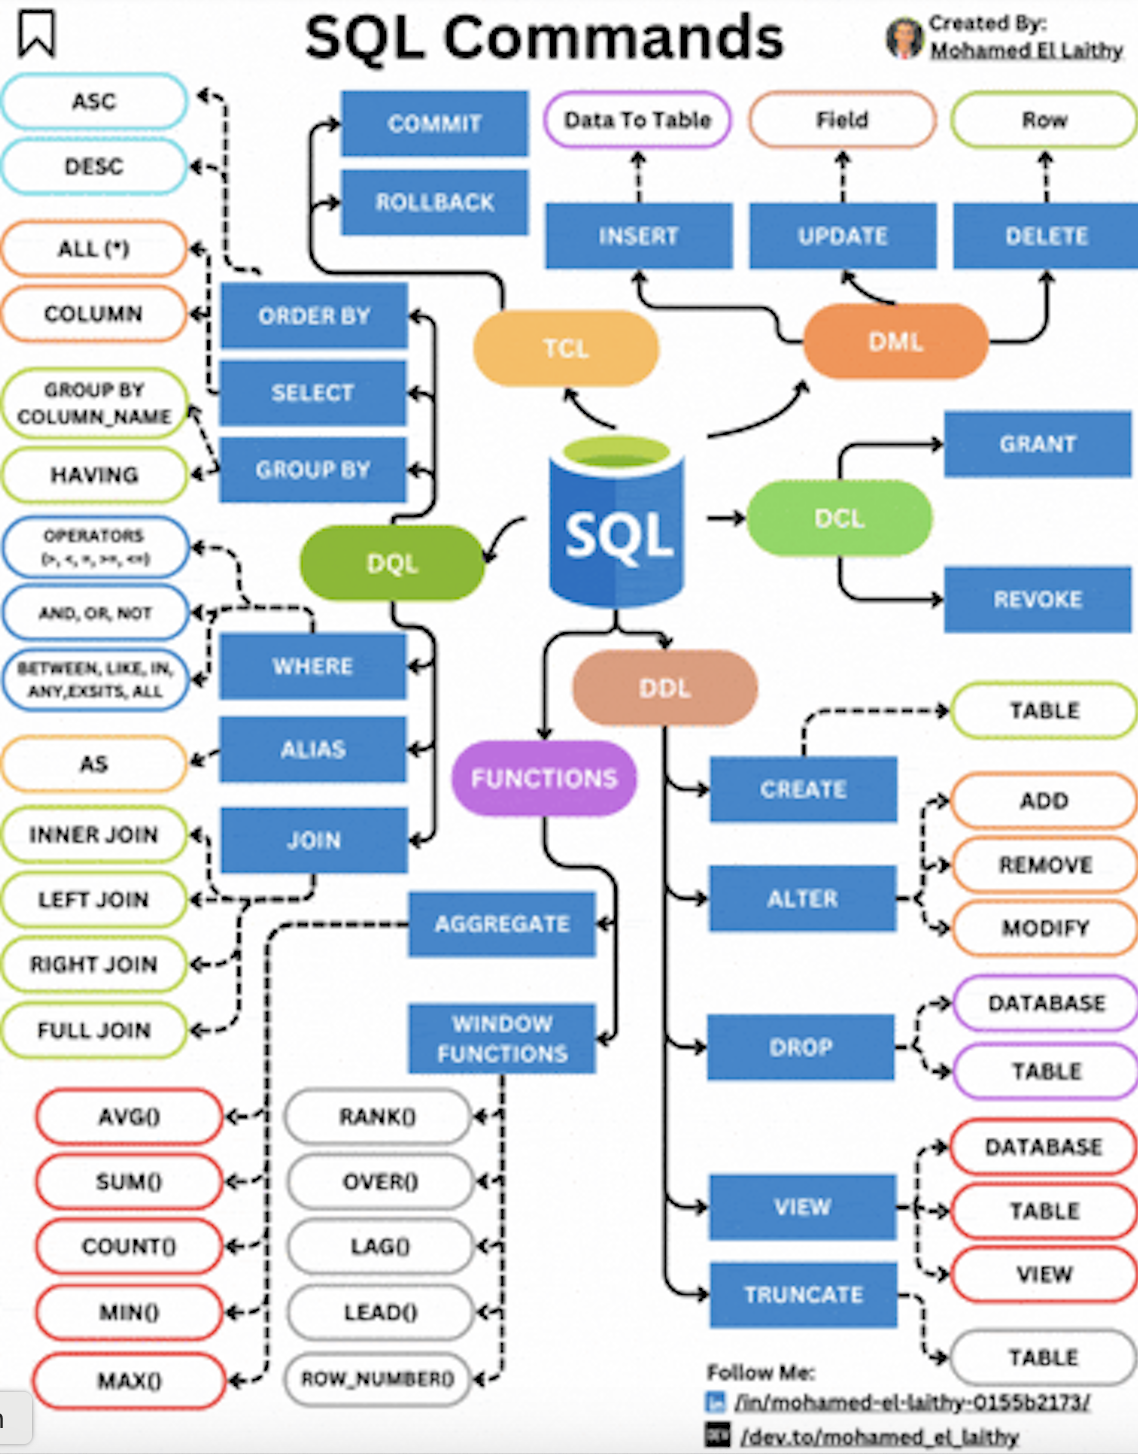
\includegraphics[scale=0.5]{schemaSQL.png} 
\end{center}

\tableofcontents

\section{SQL for Data Manipulation}

Databases store valuable information, but data is only useful if we can efficiently retrieve and manipulate it. SQL (Structured Query Language) is the standard tool for working with relational databases. This section introduces the basics of SQL, how to query data, and some practical functions that help us work with tables.

\subsection{Introduction to Databases}

\subsubsection{What is SQL?}
SQL is a language used to query and manipulate relational databases. With SQL you can:
\begin{itemize}
    \item Retrieve data
    \item Insert new data
    \item Update existing data
    \item Delete data
\end{itemize}

\subsubsection{What is Data?}
Data is a collection of facts in the form of text, numbers, or images. Businesses and applications collect data constantly, such as customer information, transactions, or sensor readings. Efficient storage and retrieval are crucial.

\subsubsection{What is a Database?}
A database is an organized repository of data.  
Relational databases store data in \textbf{tables} (rows and columns), where:
\begin{itemize}
    \item Columns describe properties of items (e.g., \texttt{FirstName}, \texttt{Email})
    \item Rows represent records or items (e.g., employees, books)
\end{itemize}

\subsubsection{Relational Database Management Systems (RDBMS)}
An RDBMS is a software system that manages relational databases. It handles:
\begin{itemize}
    \item Storing and organizing data
    \item Controlling access
    \item Querying efficiently
\end{itemize}

\paragraph{Examples:} MySQL, Oracle Database, DB2 Warehouse, DB2 on Cloud.

\subsubsection{Basic SQL Commands}
Five fundamental SQL commands are enough for most database tasks:
\begin{itemize}
    \item \texttt{CREATE TABLE} – create a new table
    \item \texttt{INSERT} – insert data into a table
    \item \texttt{SELECT} – retrieve data from a table
    \item \texttt{UPDATE} – update existing data
    \item \texttt{DELETE} – remove data from a table
\end{itemize}

\subsection{SELECT Statement}

\subsubsection{Introduction}
The \texttt{SELECT} statement is used to read data from a database.  
The result of a query is called a \textbf{result set}.  
It is part of the Data Manipulation Language (DML), which focuses on retrieving and modifying data.

\subsubsection{General Form of \texttt{SELECT}}
\begin{FormulaBox}
\texttt{SELECT <column\_name(s)> FROM <table\_name> [WHERE <condition>];}
\end{FormulaBox}

\begin{itemize}
    \item \texttt{<column\_name(s)>} – columns to retrieve (use * for all)
    \item \texttt{<table\_name>} – table to query
    \item \texttt{[WHERE <condition>]} – optional filter for rows
\end{itemize}
\paragraph{Examples}
\begin{itemize}
    \item Retrieve all columns from the table:  
\begin{verbatim}
SELECT * FROM book;
\end{verbatim}
All rows and columns of the \texttt{book} table are returned.

    \item Retrieve specific columns (\texttt{book\_id} and \texttt{title}):  
\begin{verbatim}
SELECT book_id, title FROM book;
\end{verbatim}
Only the columns \texttt{book\_id} and \texttt{title} are returned.

    \item Retrieve rows with a condition (book\_id = 'B1'):  
\begin{verbatim}
SELECT book_id, title
FROM book
WHERE book_id = 'B1';
\end{verbatim}
Only rows satisfying the condition are returned.
\end{itemize}

\subsubsection{Comparison Operators}
Common operators in the \texttt{WHERE} clause:
\begin{itemize}
    \item \texttt{=} equal to
    \item \texttt{<>} or \texttt{!=} not equal to
    \item \texttt{>} greater than
    \item \texttt{<} less than
    \item \texttt{>=} greater than or equal to
    \item \texttt{<=} less than or equal to
\end{itemize}


\subsubsection{Pattern Matching with \texttt{LIKE}}
When the exact value of a string is unknown, SQL provides the \texttt{LIKE} predicate to search for patterns within text columns.  
The \texttt{LIKE} predicate is used in the \texttt{WHERE} clause together with wildcard characters.

\begin{FormulaBox}
\texttt{SELECT <column\_name(s)> FROM <table\_name> WHERE <column> LIKE <pattern>;}
\end{FormulaBox}

\begin{itemize}
    \item \texttt{\%} – represents zero, one, or multiple characters
\end{itemize}

\paragraph{Example}
Retrieve authors whose first name starts with the letter \texttt{R}:
\begin{verbatim}
SELECT first_name
FROM author
WHERE first_name LIKE 'R%';
\end{verbatim}
All rows where the \texttt{first\_name} begins with \texttt{R} are returned.

\subsubsection{Using Ranges with \texttt{BETWEEN}}
The \texttt{BETWEEN ... AND} operator is used to filter values within a specific range.  
The boundary values are included in the result.

\begin{FormulaBox}
\texttt{SELECT <column\_name(s)> FROM <table\_name> WHERE <column> BETWEEN <value1> AND <value2>;}
\end{FormulaBox}

\paragraph{Example}
Retrieve books with a number of pages between 290 and 300:
\begin{verbatim}
SELECT title
FROM book
WHERE pages BETWEEN 290 AND 300;
\end{verbatim}
Only rows with values within the specified range are returned.


\subsubsection{Using Sets of Values with \texttt{IN}}
When filtering data based on a list of specific values, the \texttt{IN} operator can be used instead of multiple conditions.

\begin{FormulaBox}
\texttt{SELECT <column\_name(s)> FROM <table\_name> WHERE <column> IN (<value1>, <value2>, ...);}
\end{FormulaBox}

\paragraph{Example}
Retrieve authors from specific countries:
\begin{verbatim}
SELECT author_name
FROM author
WHERE country IN ('Australia', 'Brazil', 'Canada');
\end{verbatim}
Only rows matching one of the listed values are returned.

\subsubsection{Combining Conditions with \texttt{AND} and \texttt{OR}}

Multiple conditions can be combined in the \texttt{WHERE} clause using logical operators.  
Logical operators allow more precise control over which rows are included in the result set.

\begin{FormulaBox}
\texttt{SELECT <column\_name(s)> FROM <table\_name> WHERE <condition1> AND|OR <condition2>;}
\end{FormulaBox}

\begin{itemize}
    \item \texttt{AND} – returns rows only if \textbf{all} conditions are true
    \item \texttt{OR} – returns rows if \textbf{at least one} condition is true
\end{itemize}

\paragraph{Examples}
\begin{itemize}
    \item Retrieve books with more than 290 pages and less than 300 pages:
\begin{verbatim}
SELECT title
FROM book
WHERE pages > 290 AND pages < 300;
\end{verbatim}
Only rows satisfying both conditions are returned.

    \item Retrieve books with fewer than 100 pages or more than 500 pages:
\begin{verbatim}
SELECT title
FROM book
WHERE pages < 100 OR pages > 500;
\end{verbatim}
Rows satisfying either condition are returned.
\end{itemize}



\subsubsection{Sorting Results with \texttt{ORDER BY}}

By default, the result set returned by a \texttt{SELECT} statement has no guaranteed order.  
To display query results in a specific order, SQL provides the \texttt{ORDER BY} clause.

\begin{FormulaBox}
\texttt{SELECT <column\_name(s)> FROM <table\_name> ORDER BY <column\_name | column\_position> [ASC | DESC];}
\end{FormulaBox}

\begin{itemize}
    \item \texttt{ORDER BY} – specifies the column used for sorting
    \item \texttt{ASC} – ascending order (default)
    \item \texttt{DESC} – descending order
\end{itemize}

\paragraph{Examples}
\begin{itemize}
    \item Retrieve all book titles in alphabetical order:
\begin{verbatim}
SELECT title
FROM book
ORDER BY title;
\end{verbatim}
The result set is sorted in ascending (A–Z) order by default.

    \item Retrieve book titles in reverse alphabetical order:
\begin{verbatim}
SELECT title
FROM book
ORDER BY title DESC;
\end{verbatim}
The result set is sorted from Z to A.

    \item Sort books by number of pages (ascending):
\begin{verbatim}
SELECT title, pages
FROM book
ORDER BY pages;
\end{verbatim}
Books are ordered by increasing number of pages.

    \item Sort using column position instead of column name:
\begin{verbatim}
SELECT title, pages
FROM book
ORDER BY 2;
\end{verbatim}
The result set is sorted by the second column in the \texttt{SELECT} list, which is \texttt{pages}.
\end{itemize}

\begin{quote}
\textbf{Note:} When values in the sorted column are identical, SQL continues sorting using subsequent characters or values until a difference is found.
\end{quote}


\subsection{COUNT, DISTINCT, LIMIT, OFFSET}

\subsubsection{COUNT}
\texttt{COUNT} counts the number of rows matching a query.

\begin{FormulaBox}
\texttt{SELECT COUNT(<column\_name>) FROM <table\_name> [WHERE <condition>];}
\end{FormulaBox}

\paragraph{Examples:}
\begin{itemize}
    \item Count all rows: \texttt{SELECT COUNT(*) FROM MEDALS;}
    \item Count rows matching a condition: 
\begin{verbatim}
SELECT COUNT(COUNTRY) 
FROM MEDALS 
WHERE COUNTRY = 'CANADA';
\end{verbatim}
\end{itemize}

\subsubsection{DISTINCT}
\texttt{DISTINCT} removes duplicate values from the result set.

\begin{FormulaBox}
\texttt{SELECT DISTINCT <column\_name> FROM <table\_name> [WHERE <condition>];}
\end{FormulaBox}

\paragraph{Examples:}
\begin{itemize}
    \item Retrieve unique countries: \texttt{SELECT DISTINCT COUNTRY FROM MEDALS;}
    \item Unique countries with gold medals: 
\begin{verbatim}
SELECT DISTINCT COUNTRY 
FROM MEDALS 
WHERE MEDALTYPE = 'GOLD';
\end{verbatim}
\end{itemize}

\subsubsection{LIMIT}
\texttt{LIMIT} restricts the number of rows returned. LIMIT without ORDER BY always returns the \textbf{first rows}, never the last ones. 

\begin{FormulaBox}
\texttt{SELECT <column\_name(s)> FROM <table\_name> [WHERE <condition>] LIMIT <number>;}
\end{FormulaBox}

\paragraph{Examples:}
\begin{itemize}
    \item First 10 rows: \texttt{SELECT * FROM MEDALS LIMIT 10;}
    \item First 5 rows for 2018: 
\begin{verbatim}
SELECT * FROM MEDALS 
WHERE YEAR = 2018 
LIMIT 5;
\end{verbatim}
\end{itemize}
\subsubsection{OFFSET}
The \texttt{OFFSET} keyword allows you to skip a certain number of rows before starting to return results.  
It is often used together with \texttt{LIMIT} for \textbf{pagination} of query results.

\begin{FormulaBox}
\texttt{SELECT <column\_name(s)> FROM <table\_name> [WHERE <condition>] 
LIMIT <number> OFFSET <number>;}
\end{FormulaBox}

\paragraph{Examples:}
\begin{itemize}
    \item Skip the first 5 rows and retrieve the next 10 rows: 
\begin{verbatim}
SELECT * 
FROM MEDALS 
LIMIT 10 OFFSET 5;
\end{verbatim}

    \item Skip the first 20 rows for the year 2018 and retrieve the next 5 rows:
\begin{verbatim}
SELECT * 
FROM MEDALS 
WHERE YEAR = 2018 
LIMIT 5 OFFSET 20;
\end{verbatim}
\end{itemize}


\subsection{Grouping and Aggregating SELECT Results}

\subsubsection{Introduction}
Sometimes a \texttt{SELECT} query returns duplicate values or you want to summarize data.  
SQL provides keywords to \textbf{eliminate duplicates, group data, and perform aggregations}.  
The most important tools are:
\begin{itemize}
    \item \texttt{DISTINCT} – removes duplicate rows
    \item \texttt{GROUP BY} – groups rows sharing common values
    \item \texttt{HAVING} – filters groups based on conditions
\end{itemize}

\subsubsection{Eliminating Duplicates with \texttt{DISTINCT}}
The \texttt{DISTINCT} keyword reduces a result set to \textbf{unique values only}.

\begin{FormulaBox}
\texttt{SELECT DISTINCT <column\_name(s)> FROM <table\_name> [ORDER BY <column>];}
\end{FormulaBox}

\paragraph{Example}
Retrieve a list of unique countries for authors:
\begin{verbatim}
SELECT DISTINCT country
FROM author
ORDER BY 1;
\end{verbatim}
Only unique countries are returned, sorted alphabetically.

\subsubsection{Grouping Data with \texttt{GROUP BY}}
The \texttt{GROUP BY} clause groups rows that have the same values in one or more columns.  
It is often used with \textbf{aggregate functions} like \texttt{COUNT}, \texttt{SUM}, or \texttt{AVG}.

\begin{FormulaBox}
\texttt{SELECT <column\_name>, AGGREGATE\_FUNCTION(<column>) 
FROM <table\_name> 
GROUP BY <column\_name>;}
\end{FormulaBox}

\paragraph{Example}
Count the number of authors from each country:
\begin{verbatim}
SELECT country, COUNT(*)
FROM author
GROUP BY country;
\end{verbatim}
The result set shows each country and the number of authors from that country.  
By default, the second column is named after the aggregate function (e.g., "COUNT(*)").  

\subsubsection{Renaming Columns with \texttt{AS}}
Use \texttt{AS} to assign a \textbf{meaningful name} to a derived column:

\begin{FormulaBox}
\texttt{SELECT <column>, AGGREGATE\_FUNCTION(<column>) AS <alias>
FROM <table>
GROUP BY <column>;}
\end{FormulaBox}

\paragraph{Example}
Rename the count column to \texttt{AuthorCount}:
\begin{verbatim}
SELECT country, COUNT(*) AS AuthorCount
FROM author
GROUP BY country;
\end{verbatim}

\subsubsection{Filtering Groups with \texttt{HAVING}}
The \texttt{HAVING} clause sets conditions \textbf{on groups}, unlike \texttt{WHERE}, which filters individual rows.  

\begin{FormulaBox}
\texttt{SELECT <column>, AGGREGATE\_FUNCTION(<column>) AS <alias>
FROM <table>
GROUP BY <column>
HAVING <aggregate\_condition>;}
\end{FormulaBox}

\paragraph{Example}
Only show countries with more than 4 authors:
\begin{verbatim}
SELECT country, COUNT(*) AS AuthorCount
FROM author
GROUP BY country
HAVING COUNT(*) > 4;
\end{verbatim}
Result: Only countries with five or more authors are returned (e.g., China, India).




\subsection{INSERT Statement}

\subsubsection{Introduction}
The \texttt{INSERT} statement is used to add new rows to a relational database table.  
It is part of the \textbf{Data Manipulation Language (DML)}, which allows you to read and modify data.  
After a table is created, it needs to be populated with data. There are \textbf{two main ways} to add rows:
\begin{itemize}
    \item Insert \textbf{one row at a time}
    \item Insert \textbf{multiple rows at once}
\end{itemize}


\subsubsection{General Form of \texttt{INSERT}}
\begin{FormulaBox}
\texttt{INSERT INTO <table\_name> (<column\_name(s)>) VALUES (<value(s)>); }
\end{FormulaBox}

\begin{itemize}
    \item \texttt{<table\_name>} – the table you want to insert data into  
    \item \texttt{<column\_name(s)>} – list of columns being populated  
    \item \texttt{<value(s)>} – values for each column (order must match column list)  
\end{itemize}
\paragraph{Examples}
\begin{itemize}
    \item Insert a single row into the \texttt{author} table:  
\begin{verbatim}
INSERT INTO author (author_id, last_name, first_name, email, city, country)
VALUES ('A1', 'Chong', 'Raul', 'RFC@IBM.com', 'Toronto', 'CA');
\end{verbatim}

    \item Insert multiple rows at once:  
\begin{verbatim}
INSERT INTO author (author_id, last_name, first_name, email, city, country)
VALUES 
('A1', 'Chong', 'Raul', 'RFC@IBM.com', 'Toronto', 'CA'),
('A2', 'Ahuja', 'Rav', 'RA@IBM.com', 'Vancouver', 'CA');
\end{verbatim}
\end{itemize}

\paragraph{Notes:}
- The number of values in each row must match the number of columns specified  
- Multiple rows are separated by commas inside the \texttt{VALUES} clause



\subsection{UPDATE and DELETE Statements}

\subsubsection{Introduction}
After a table is created and populated with data, you may want to modify or remove rows.  
\\
- The \texttt{UPDATE} statement is used to alter existing data. 
\\ 
- The \texttt{DELETE} statement is used to remove rows from a table.  
\\
Both are part of the Data Manipulation Language (DML).  
It is important to always use the WHERE clause; without it, all rows in the table may be affected.

\subsubsection{General Form of \texttt{UPDATE}}
\begin{FormulaBox}
\texttt{UPDATE <table\_name> SET <column\_name> = <value> [, ...] [WHERE <condition>];}
\end{FormulaBox}

\paragraph{Parameters:}
\begin{itemize}
    \item \texttt{<table\_name>} – the table to update  
    \item \texttt{<column\_name> = <value>} – column(s) and new values  
    \item \texttt{[WHERE <condition>]} – optional filter to update specific rows
\end{itemize}

\subsubsection{General Form of \texttt{DELETE}}
\begin{FormulaBox}
\texttt{DELETE FROM <table\_name> [WHERE <condition>];}
\end{FormulaBox}

\paragraph{Parameters:}
\begin{itemize}
    \item \texttt{<table\_name>} – the table to delete rows from  
    \item \texttt{[WHERE <condition>]} – optional filter to delete specific rows
\end{itemize}


\paragraph{Examples}
\begin{itemize}
    \item Update the first and last name of the author with \texttt{AUTHOR\_ID = 'A2'}:  
\begin{verbatim}
UPDATE author
SET last_name = 'Katta', first_name = 'Lakshmi'
WHERE author_id = 'A2';
\end{verbatim}

    \item Delete authors with \texttt{AUTHOR\_ID = 'A2'} or \texttt{'A3'}:  
\begin{verbatim}
DELETE FROM author
WHERE author_id IN ('A2', 'A3');
\end{verbatim}
\paragraph{Note:} Always include the \textbf{WHERE clause}.  
Without it:  
- \texttt{UPDATE} will change all rows  
- \texttt{DELETE} will remove all rows
\end{itemize}

\newpage
\section{Functions, Multiple Tables and Sub-queries}


\subsection{Introduction}
SQL provides built-in functions that allow operations to be performed \textbf{directly in the database}, reducing the amount of data transferred to applications and improving efficiency.  

Functions can operate on:
\begin{itemize}
    \item Entire columns (aggregate functions)
    \item Individual values (scalar functions)
    \item Strings (string functions)
\end{itemize}

Using functions inside SQL queries is more efficient than retrieving data first and performing operations in an application.

\subsection{Aggregate Functions}
Aggregate functions take a collection of values (typically in a column) and return a \textbf{single value}.  

\begin{FormulaBox}
\texttt{SELECT AGGREGATE\_FUNCTION(<column>) [AS <alias>] FROM <table\_name> [WHERE <condition>];}
\end{FormulaBox}

\paragraph{Common Aggregate Functions}
\begin{itemize}
    \item \texttt{SUM(<column>)} – returns the sum of all values
    \item \texttt{MIN(<column>)} – returns the minimum value
    \item \texttt{MAX(<column>)} – returns the maximum value
    \item \texttt{AVG(<column>)} – returns the average value
    \item \texttt{COUNT(<column>)} – returns the number of rows
\end{itemize}

\paragraph{Examples}  
Using the \texttt{PETRESCUE} table with columns \texttt{ID, ANIMAL, QUANTITY, COST, RESCUE\_DATE}:
\begin{itemize}
    \item Total cost of all rescues:
\begin{verbatim}
SELECT SUM(COST) AS SUM_OF_COST
FROM PETRESCUE;
\end{verbatim}

    \item Minimum ID for dog rescues:
\begin{verbatim}
SELECT MIN(ID)
FROM PETRESCUE
WHERE ANIMAL = 'Dog';
\end{verbatim}

    \item Maximum quantity in a single rescue:
\begin{verbatim}
SELECT MAX(QUANTITY)
FROM PETRESCUE;
\end{verbatim}

    \item Average cost per dog (cost divided by quantity):
\begin{verbatim}
SELECT AVG(COST / QUANTITY)
FROM PETRESCUE
WHERE ANIMAL = 'Dog';
\end{verbatim}
\end{itemize}

\subsection{Scalar Functions}
Scalar functions perform operations on \textbf{individual values} in a column.  

\begin{FormulaBox}
\texttt{SELECT SCALAR\_FUNCTION(<column>) FROM <table\_name> [WHERE <condition>];}
\end{FormulaBox}
\paragraph{Numeric Functions}
\begin{itemize}
    \item \texttt{ROUND(column, n)} – rounds a numeric value to n decimal places  
    \item \texttt{CEIL(column)} – returns the smallest integer greater than or equal to the value  
    \item \texttt{FLOOR(column)} – returns the largest integer less than or equal to the value  
    \item \texttt{ABS(column)} – returns the absolute value  
\end{itemize}
\paragraph{Examples}
\begin{itemize}
    \item Round cost to nearest integer:
\begin{verbatim}
SELECT ROUND(COST)
FROM PETRESCUE;
\end{verbatim}

    \item Retrieve lowercase animal names for cats:
\begin{verbatim}
SELECT *
FROM PETRESCUE
WHERE LOWER(ANIMAL) = 'cat';
\end{verbatim}
\end{itemize}

\subsection{String Functions}
String functions operate on character or text columns (\texttt{CHAR, VARCHAR}).  

\begin{FormulaBox}
\texttt{SELECT STRING\_FUNCTION(<column>) FROM <table\_name> [WHERE <condition>];}
\end{FormulaBox}

\paragraph{Common String Functions}
\begin{itemize}
    \item \texttt{LENGTH(<column>)} – returns the length of the string
    \item \texttt{UPPER(<column>)} – converts string to uppercase
    \item \texttt{LOWER(<column>)} – converts string to lowercase
\end{itemize}

\paragraph{Examples}
\begin{itemize}
    \item Length of each animal name:
\begin{verbatim}
SELECT LENGTH(ANIMAL)
FROM PETRESCUE;
\end{verbatim}

    \item Animal names in uppercase:
\begin{verbatim}
SELECT UPPER(ANIMAL)
FROM PETRESCUE;
\end{verbatim}

    \item Unique uppercase animal names:
\begin{verbatim}
SELECT DISTINCT UPPER(ANIMAL)
FROM PETRESCUE;
\end{verbatim}
\end{itemize}

\subsection{Date and Time Functions}

\subsubsection{Introduction}
SQL provides special data types and functions to work with \textbf{dates and times}.  
Most databases support the following types:
\begin{itemize}
    \item \texttt{DATE} – 8 digits, format \texttt{YYYYMMDD}
    \item \texttt{TIME} – 6 digits, format \texttt{HHMMSS}
    \item \texttt{TIMESTAMP} – 20 digits, format \texttt{YYYYMMDDHHMMSSZZZZZZ} (\texttt{ZZZZZZ} = microseconds)
\end{itemize}

Date and time functions can be used to extract specific components, perform calculations, and filter data.

\subsubsection{Extracting Date and Time Components}
Functions exist to extract various parts of a date or time:
\begin{itemize}
    \item \texttt{DAY()} – day of the month
    \item \texttt{MONTH()} – month of the year
    \item \texttt{YEAR()} – year
    \item \texttt{WEEK()} – week number
    \item \texttt{HOUR()}, \texttt{MINUTE()}, \texttt{SECOND()} – time components
    \item \texttt{DAYOFWEEK()} – day of the week
    \item \texttt{DAYOFYEAR()} – day of the year
\end{itemize}

\begin{FormulaBox}
\texttt{SELECT FUNCTION(<column>) FROM <table\_name> [WHERE <condition>];}
\end{FormulaBox}

\paragraph{Examples}
\begin{itemize}
    \item Extract day from rescue dates for cats:
\begin{verbatim}
SELECT DAY(rescue_date)
FROM PETRESCUE
WHERE ANIMAL = 'Cat';
\end{verbatim}

    \item Count rescues in the month of May (month = 5):
\begin{verbatim}
SELECT COUNT(*)
FROM PETRESCUE
WHERE MONTH(rescue_date) = 5;
\end{verbatim}
\end{itemize}

\subsubsection{Date and Time Arithmetic}
SQL allows arithmetic with dates and times to calculate intervals or durations.

\begin{FormulaBox}
\texttt{SELECT <column> + INTERVAL <number> <unit> FROM <table\_name>;}
\end{FormulaBox}
\paragraph{Common Functions}
\begin{itemize}
    \item \texttt{DATE\_ADD(date, INTERVAL n unit)} – adds time to a date
    \item \texttt{DATE\_SUB(date, INTERVAL n unit)} – subtracts time from a date
    \item \texttt{DATEDIFF(date1, date2)} – difference in days between two dates
    \item \texttt{TIMEDIFF(time1, time2)} – difference between two times
    \item \texttt{NOW()} – current date and time
    \item \texttt{CURDATE()} – current date only
    \item \texttt{CURTIME()} – current time only
    \item \texttt{EXTRACT(unit FROM date)} – extracts a part of the date/time (e.g., year, month, day)
    \item \texttt{FROM\_DAYS(n)} – converts a number of days into a date
\end{itemize}
\paragraph{Examples}
\begin{itemize}
    \item Date three days after each rescue:
\begin{verbatim}
SELECT DATE_ADD(rescue_date, INTERVAL 3 DAY)
FROM PETRESCUE;
\end{verbatim}

    \item Date two weeks before each rescue:
\begin{verbatim}
SELECT DATE_SUB(rescue_date, INTERVAL 2 WEEK)
FROM PETRESCUE;
\end{verbatim}

    \item Days elapsed since each rescue until today:
\begin{verbatim}
SELECT DATEDIFF(CURDATE(), rescue_date)
FROM PETRESCUE;
\end{verbatim}

    \item Time difference between two columns:
\begin{verbatim}
SELECT TIMEDIFF(end_time, start_time)
FROM PETRESCUE;
\end{verbatim}

    \item Extract month and year from rescue date:
\begin{verbatim}
SELECT EXTRACT(MONTH FROM rescue_date), EXTRACT(YEAR FROM rescue_date)
FROM PETRESCUE;
\end{verbatim}
\end{itemize}

\paragraph{Notes}
\begin{itemize}
    \item Date and time functions can also be used in the \texttt{WHERE} clause.
    \item Arithmetic can be performed using addition/subtraction of intervals or timestamps.
    \item These functions help filter, calculate, and analyze data based on time periods.
\end{itemize}


\subsection{Subqueries (Nested SELECT Statements)}

A \textbf{subquery} (also called a \textbf{nested SELECT}) is a query placed inside another SQL query.  
Subqueries are enclosed in parentheses and allow more powerful data retrieval.
A subquery can appear in:
\begin{itemize}
    \item the \texttt{WHERE} clause
    \item the \texttt{SELECT} list (column expressions)
    \item the \texttt{FROM} clause (derived tables)
\end{itemize}

\subsubsection{Subquery in the WHERE Clause}

\begin{FormulaBox}
\texttt{SELECT <column\_name(s)> FROM <table\_name> 
WHERE <column> <operator> (SELECT <aggregate\_function> FROM <table\_name>);}
\end{FormulaBox}

\paragraph{Example :}
Retrieve employees who earn more than the average salary:
\begin{verbatim}
SELECT employee_id, first_name, last_name, salary
FROM employees
WHERE salary > (
    SELECT AVG(salary)
    FROM employees
);
\end{verbatim}

\subsubsection{Subquery in the SELECT List (Column Expression)}

\begin{FormulaBox}
\texttt{SELECT <column>, (SELECT <aggregate\_function> FROM <table>) AS <alias>
FROM <table\_name>;}
\end{FormulaBox}

\paragraph{Example :}
Display each employee's salary along with the average salary:
\begin{verbatim}
SELECT employee_id, salary,
       (SELECT AVG(salary) FROM employees) AS avg_salary
FROM employees;
\end{verbatim}

\subsubsection{Subquery in the FROM Clause (Derived Table)}

\begin{FormulaBox}
\texttt{SELECT <column\_name(s)>
FROM (SELECT <column\_name(s)> FROM <table\_name>) AS <alias>;}
\end{FormulaBox}

\paragraph{Example :}
Create a derived table with non-sensitive employee data:
\begin{verbatim}
SELECT *
FROM (
    SELECT employee_id, first_name, last_name, department_id
    FROM employees
) AS employee_info;
\end{verbatim}

\paragraph{Notes on Subqueries :}

\begin{itemize}
    \item Subqueries must be enclosed in parentheses
    \item Aggregate functions are often used inside subqueries
    \item Subqueries in the \texttt{FROM} clause must have an alias
\end{itemize}



\subsection{Accessing Multiple Tables: Using Subqueries with Multiple Tables}

A subquery can be used to filter rows in one table based on data stored in another table.

\begin{FormulaBox}
\texttt{SELECT <column\_name(s)> FROM <table1>
WHERE <column> IN (SELECT <column> FROM <table2>);}
\end{FormulaBox}

\paragraph{Examples}

\begin{itemize}
    \item Retrieve employees whose department exists in the \texttt{departments} table:
\begin{verbatim}
SELECT *
FROM employees
WHERE dep_id IN (
    SELECT dep_id
    FROM departments
);
\end{verbatim}

    \item Retrieve employees working in a specific location:
\begin{verbatim}
SELECT *
FROM employees
WHERE dep_id IN (
    SELECT dep_id
    FROM departments
    WHERE loc_id = 'L0002'
);
\end{verbatim}

    \item Retrieve department details for employees earning more than 70,000:
\begin{verbatim}
SELECT dep_id, dep_name
FROM departments
WHERE dep_id IN (
    SELECT dep_id
    FROM employees
    WHERE salary > 70000
);
\end{verbatim}
\end{itemize}

\subsection{Accessing Multiple Tables: Implicit Joins (Multiple Tables in FROM Clause)}

Multiple tables can be accessed by listing them in the \texttt{FROM} clause.  
This creates a join between tables without explicitly using a JOIN keyword.

\begin{FormulaBox}
\texttt{SELECT <column\_name(s)> FROM <table1>, <table2> [WHERE <join\_condition>];}
\end{FormulaBox}

\paragraph{Examples}

\begin{itemize}
    \item Cartesian product (no condition specified), \textbf{Cross Join}:
\begin{verbatim}
SELECT *
FROM employees, departments;
\end{verbatim}

    \item Join employees with their departments using a condition, \textbf{Inner Join}:
\begin{verbatim}
SELECT *
FROM employees, departments
WHERE employees.dep_id = departments.dep_id;
\end{verbatim}

    \item Using table \textbf{aliases} for readability:
\begin{verbatim}
SELECT *
FROM employees E, departments D
WHERE E.dep_id = D.dep_id;
\end{verbatim}

    \item Retrieve employee ID and department name:
\begin{verbatim}
SELECT E.emp_id, D.dep_name
FROM employees E, departments D
WHERE E.dep_id = D.dep_id;
\end{verbatim}
\end{itemize}
\textbf{The aliases notation and the notations form the two last examples are very usefull}
\subsubsection{Notes}

\begin{itemize}
    \item Always qualify column names when multiple tables are used
    \item Table aliases make queries shorter and easier to read
    \item Implicit joins are logically equivalent to INNER JOINs when a matching condition is specified
\end{itemize}


\subsection{Accessing Multiple Tables: JOIN Operations}

SQL provides explicit \texttt{JOIN} operators to combine rows from two or more tables based on related columns.  
Using JOINs improves readability and makes query intent clearer compared to implicit joins.

\begin{FormulaBox}
\texttt{SELECT <column\_name(s)> 
FROM <table1> <JOIN\_TYPE> <table2>
ON <join\_condition>;}
\end{FormulaBox}

\subsubsection{INNER JOIN}

Returns only rows that have matching values in both tables.

\begin{verbatim}
SELECT E.emp_id, D.dep_name
FROM employees E
INNER JOIN departments D
ON E.dep_id = D.dep_id;
\end{verbatim}

\textbf{Result:} Rows with matching department IDs in both tables.

\subsubsection{CROSS JOIN}

Returns the Cartesian product of both tables (every row from the first table combined with every row from the second table).

\begin{verbatim}
SELECT *
FROM employees
CROSS JOIN departments;
\end{verbatim}

\textbf{Result:} Number of rows = rows in employees × rows in departments.

\subsubsection{LEFT (OUTER) JOIN}

Returns all rows from the left table and matching rows from the right table.  
Non-matching rows from the right table return \texttt{NULL} values.

\begin{verbatim}
SELECT E.emp_id, D.dep_name
FROM employees E
LEFT JOIN departments D
ON E.dep_id = D.dep_id;
\end{verbatim}

\subsubsection{RIGHT (OUTER) JOIN}

Returns all rows from the right table and matching rows from the left table.  
Non-matching rows from the left table return \texttt{NULL} values.

\begin{verbatim}
SELECT E.emp_id, D.dep_name
FROM employees E
RIGHT JOIN departments D
ON E.dep_id = D.dep_id;
\end{verbatim}

\subsubsection{FULL (OUTER) JOIN}

Returns all rows from both tables.  
Rows without matches on either side contain \texttt{NULL} values.

\begin{verbatim}
SELECT E.emp_id, D.dep_name
FROM employees E
FULL JOIN departments D
ON E.dep_id = D.dep_id;
\end{verbatim}

\subsubsection{SELF JOIN}

A table is joined with itself.  
Useful for hierarchical or recursive relationships (e.g., employees and managers).

\begin{verbatim}
SELECT E.emp_id, M.emp_id AS manager_id
FROM employees E
LEFT JOIN employees M
ON E.manager_id = M.emp_id;
\end{verbatim}

\subsubsection{NATURAL JOIN}

Automatically joins tables based on columns with the same name and compatible data types.  
No \texttt{ON} clause is required.

\begin{verbatim}
SELECT *
FROM employees
NATURAL JOIN departments;
\end{verbatim}
\begin{quote}
\textbf{Note:} \texttt{NATURAL JOIN} should be used with caution, as it depends on column naming conventions.
\end{quote}

\subsubsection{Summary of JOIN Types}

\begin{itemize}
    \item \texttt{INNER JOIN} – matching rows only
    \item \texttt{CROSS JOIN} – all combinations of rows
    \item \texttt{LEFT JOIN} – all rows from left table
    \item \texttt{RIGHT JOIN} – all rows from right table
    \item \texttt{FULL JOIN} – all rows from both tables
    \item \texttt{SELF JOIN} – table joined with itself
    \item \texttt{NATURAL JOIN} – automatic join on same-named columns
\end{itemize}






























\newpage

\section{Types of SQL Statements and DDL}

SQL statements interact with \textbf{Entities} (tables), \textbf{Attributes} (columns), and their \textbf{Tuples} (rows). These statements generally fall into two main categories: Data Definition Language (DDL) and Data Manipulation Language (DML).

\subsection{Database Models and Design}

Before writing SQL code, databases are designed using models. The most common are the Relational Model and the Entity-Relationship (ER) Model.

\subsubsection{The Relational Model}
The relational model is the most widely used data model because it offers \textbf{Data Independence}:
\begin{itemize}
    \item \textbf{Logical Data Independence:} Changing the schema (structure) does not affect the data.
    \item \textbf{Physical Data Independence:} Changing how data is stored physically does not affect the logical structure.
\end{itemize}

\subsubsection{Entity-Relationship (ER) Model}
The ER model is a tool used to design relational databases. It visualizes data as a collection of \textbf{Entities and Attributes}.

\begin{itemize}
    \item \textbf{Entity (Table):} An object that exists independently (Person, Place, Thing). 
    \item \textbf{Attribute (Column):} Data elements that characterize the entity.
\end{itemize}

\begin{center}
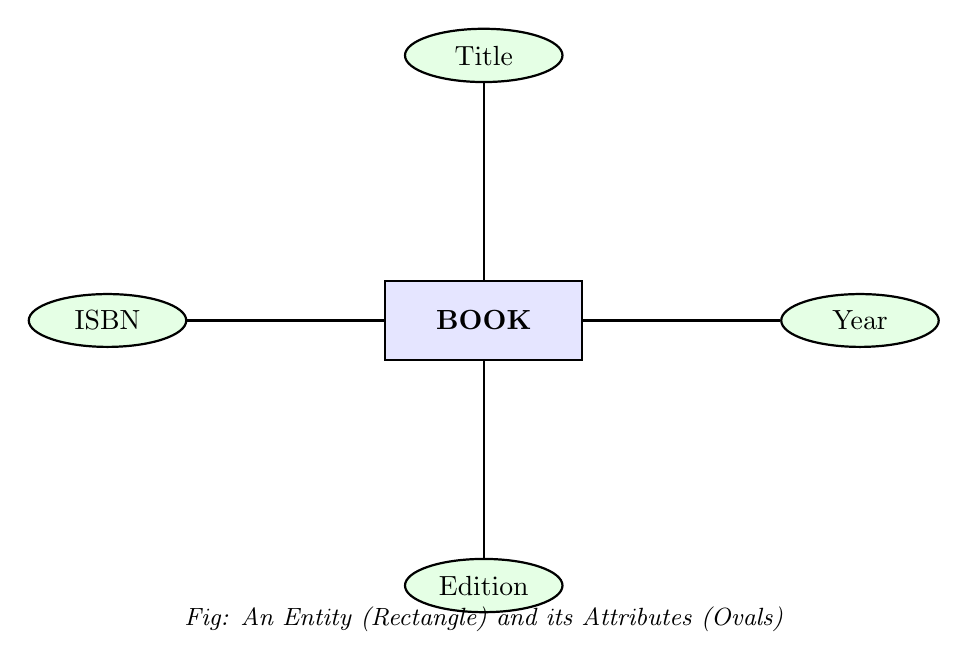
\begin{tikzpicture}[
    node distance=2.5cm,
    entity/.style={rectangle, draw=black, thick, minimum width=2.5cm, minimum height=1cm, fill=blue!10},
    attribute/.style={ellipse, draw=black, thick, minimum width=2cm, fill=green!10},
    line/.style={-, thick}
]

    % Entity
    \node[entity] (book) {\textbf{BOOK}};

    % Attributes
    \node[attribute, above=of book] (title) {Title};
    \node[attribute, left=of book] (isbn) {ISBN};
    \node[attribute, right=of book] (year) {Year};
    \node[attribute, below=of book] (edition) {Edition};

    % Connections
    \draw[line] (book) -- (title);
    \draw[line] (book) -- (isbn);
    \draw[line] (book) -- (year);
    \draw[line] (book) -- (edition);
    
    \node[below=3cm of book, align=center, font=\small\itshape] {Fig: An Entity (Rectangle) and its Attributes (Ovals)};

\end{tikzpicture}
\end{center}

\subsubsection{Mapping Entities to Tables}
Once the design is complete, we map the ER diagram to a Relational Database:

\begin{center}
\begin{tabular}{| c | c | c |}
\hline
\textbf{ER Model} & \textbf{Map To} & \textbf{Relational Database} \\
\hline
Entity & $\rightarrow$ & \textbf{Table} \\
\hline
Attribute & $\rightarrow$ & \textbf{Column} \\
\hline
Instance & $\rightarrow$ & \textbf{Row (Tuple)} \\
\hline
\end{tabular}
\end{center}

During this phase, we choose specific data types for columns (e.g., using \texttt{VARCHAR} for variable titles or \texttt{CHAR} for fixed-length codes like ISBNs which may contain dashes).

\subsubsection{Primary and Foreign Keys}
Keys are fundamental to the relational model for identity and relationships.

\begin{itemize}
    \item \textbf{Primary Key (PK):} A column (or set of columns) that \textbf{uniquely identifies} each row in a table. It prevents duplicate data.
    \item \textbf{Foreign Key (FK):} A primary key from one table that appears in another table. It creates a \textbf{link} (relationship) between the two tables.
\end{itemize}

\subsection{Relational Model Constraints}

To maintain data integrity in a relational database, the relational model defines three essential types of constraints. These constraints ensure that data remains accurate, consistent, and logically connected.

\begin{itemize}

    \item \textbf{Entity Integrity:}  
    Ensures that each table has a \textbf{Primary Key} that uniquely identifies every row.  
    Primary key values must be \textbf{unique} and \textbf{NOT NULL}, preventing duplicate or unidentified records.

    \item \textbf{Referential Integrity:}  
    Ensures that relationships between tables remain valid by enforcing \textbf{Foreign Key} constraints.  
    A foreign key value must reference an existing primary key in another table, preventing orphan or invalid references.

    \item \textbf{Domain Integrity:}  
    Ensures that all values stored in a column are valid according to defined rules such as:
    data type, format, allowed range, and nullability.  
    This is enforced using constraints like \texttt{CHECK} and \texttt{NOT NULL}.

\end{itemize}

Together, these constraints preserve the reliability and correctness of data in a relational database.

\subsection{Categories of SQL Statements}

\subsubsection{Data Definition Language (DDL)}
DDL statements are used to define, change, or drop database objects such as tables. They manage the structure of the database.

Common DDL statements include:
\begin{itemize}
    \item \texttt{CREATE}: Used for creating tables and defining their columns.
    \item \texttt{ALTER}: Used for modifying table structures (e.g., adding/dropping columns, changing data types).
    \item \texttt{TRUNCATE}: Used for deleting all data in a table but keeping the table structure itself.
    \item \texttt{DROP}: Used for deleting tables entirely (structure and data).
\end{itemize}

\subsubsection{Data Manipulation Language (DML)}
DML statements are used to read and modify data within existing tables. These operations are often referred to as \textbf{CRUD} (Create, Read, Update, Delete).

Common DML statements include:
\begin{itemize}
    \item \texttt{INSERT} (Create): Inserts a row or several rows of data.
    \item \texttt{SELECT} (Read): Reads or selects rows from a table.
    \item \texttt{UPDATE} (Update): Edits existing rows in a table.
    \item \texttt{DELETE} (Delete): Removes rows of data from a table.
\end{itemize}

\subsection{The CREATE TABLE Statement}

The \texttt{CREATE TABLE} statement is the most common DDL command. It allows you to define an entity (table name) and its attributes (columns) with specific data types and constraints.



\subsubsection{General Syntax}
\begin{FormulaBox}
\texttt{CREATE TABLE <table\_name> ( \\
\hspace*{1em} <column\_1> <datatype> [optional\_constraints], \\
\hspace*{1em} <column\_2> <datatype> [optional\_constraints], \\
\hspace*{1em} ... \\
);}
\end{FormulaBox}

\subsubsection{Data Types and Constraints}
When defining columns, you must specify the data type:
\begin{itemize}
    \item \texttt{CHAR(n)}: A character string of fixed length $n$.
    \item \texttt{VARCHAR(n)}: A character string of variable length (up to $n$ characters).
    \item \texttt{INTEGER} (or \texttt{INT}): Stores whole numbers (e.g., 1, 50, -10).
    \item \texttt{DECIMAL(p,s)}: Stores exact numeric values with fixed precision $p$ (total digits) and scale $s$ (decimal digits), often used for currency.
    \item \texttt{FLOAT} / \texttt{DOUBLE}: Stores approximate numeric values (floating-point numbers) for scientific calculations.
    \item \texttt{DATE}: Stores a date value (format: YYYY-MM-DD).
    \item \texttt{TIME}: Stores a time value (format: HH:MM:SS).
    \item \texttt{TIMESTAMP}: Stores both date and time (format: YYYY-MM-DD HH:MM:SS).
    \item \texttt{BOOLEAN}: Stores boolean values (\texttt{TRUE} or \texttt{FALSE}).
\end{itemize}
You can also apply constraints to ensure data integrity:
\begin{itemize}
    \item \texttt{PRIMARY KEY}: Uniquely identifies each tuple (row). No duplicate values allowed.
    \item \texttt{NOT NULL}: Ensures the column cannot be empty (must contain a value).
    \item \texttt{UNIQUE}: Ensures all values in a column are different.
    \item \texttt{FOREIGN KEY}: Ensures referential integrity by linking to a Primary Key in another table.
\end{itemize}

\subsubsection{Example: Creating an Author Table}
In a Library database, we might create a table for the \texttt{AUTHOR} entity.
\begin{itemize}
    \item \textbf{Table Name:} author
    \item \textbf{Columns:} author\_id, lastname, firstname, email, city, country
    \item \textbf{Constraints:} author\_id is the Primary Key; names cannot be null.
\end{itemize}

\begin{verbatim}
CREATE TABLE author (
    author_id CHAR(2) PRIMARY KEY NOT NULL,
    lastname VARCHAR(15) NOT NULL,
    firstname VARCHAR(15) NOT NULL,
    email VARCHAR(40),
    city VARCHAR(15),
    country CHAR(2)
);
\end{verbatim}
Executing this statement creates the structure in the database, ready to receive data via DML statements.


\subsection{Modifying and Deleting Tables (ALTER, DROP, TRUNCATE)}

While \texttt{CREATE} defines the initial structure, requirements often change. SQL provides specific DDL statements to modify existing structures or remove them entirely.

\subsubsection{ALTER TABLE Statement}
The \texttt{ALTER TABLE} statement is used to change the structure of an existing table. Unlike \texttt{CREATE TABLE}, it does not use parentheses to enclose parameters.

\begin{FormulaBox}
\texttt{ALTER TABLE <table\_name> <action> <column\_name> [options];}
\end{FormulaBox}

Common actions include:

\begin{itemize}

    \item \textbf{ADD COLUMN}: Adds a new attribute to the table.
    \begin{verbatim}
    ALTER TABLE author ADD COLUMN telephone_number BIGINT;
    \end{verbatim}

    \item \textbf{MODIFY / ALTER COLUMN}: Changes the data type or constraints of an existing column.
    \begin{verbatim}
    ALTER TABLE author MODIFY telephone_number CHAR(20);
    \end{verbatim}

    \item \textbf{DROP COLUMN}: Removes a column from the table structure.
    \begin{verbatim}
    ALTER TABLE author DROP COLUMN telephone_number;
    \end{verbatim}

    \item \textbf{RENAME COLUMN}: Changes the name of a column.
    \begin{verbatim}
    ALTER TABLE author RENAME COLUMN lastname TO last_name;
    \end{verbatim}

    \item \textbf{ADD/DROP CONSTRAINT}: Removes an existing constraint.
    \begin{verbatim}
    ALTER TABLE author DROP CONSTRAINT unique_email;
    ALTER TABLE author ADD CONSTRAINT unique_email UNIQUE (email);
    \end{verbatim}


    \item \textbf{ADD/DROP PRIMARY KEY/FOREIGN KEY}: Removes a key constraint.
    \begin{verbatim}
    ALTER TABLE author DROP PRIMARY KEY;
    ALTER TABLE author ADD PRIMARY KEY (author_id);
    \end{verbatim}

    \item \textbf{SET DEFAULT}: Assigns a default value to a column.
    \begin{verbatim}
    ALTER TABLE author ALTER COLUMN country SET DEFAULT 'US';
    \end{verbatim}

    \item \textbf{DROP DEFAULT}: Removes the default value of a column.
    \begin{verbatim}
    ALTER TABLE author ALTER COLUMN country DROP DEFAULT;
    \end{verbatim}

    \item \textbf{RENAME TABLE}: Changes the table name.
    \begin{verbatim}
    ALTER TABLE author RENAME TO writer;
    \end{verbatim}

\end{itemize}
\begin{quote}
    \textbf{Warning:} Altering a data type with existing data can cause errors if the data is incompatible (e.g., converting a \texttt{CHAR} column containing letters into a numeric type).
\end{quote}



\subsubsection{DROP TABLE Statement}
The \texttt{DROP TABLE} statement is used to remove a table definition and all its data from the database permanently.

\begin{FormulaBox}
\texttt{DROP TABLE <table\_name>;}
\end{FormulaBox}


\paragraph{Example:}
\begin{verbatim}
    DROP TABLE author;
\end{verbatim}
\textit{Effect:}
\begin{itemize}
    \item The entire table definition is deleted.
    \item All rows (data) are permanently lost.
    \item Indexes, constraints, and relationships associated with the table are also removed.
    \item The table no longer exists and must be recreated to be used again.
\end{itemize}
\textbf{Important:} \texttt{DROP TABLE} is irreversible and cannot be rolled back in most database systems.


\subsubsection{TRUNCATE TABLE Statement}
The \texttt{TRUNCATE} statement is used to delete all rows within a table while keeping the table structure (columns/types) intact. 

\begin{FormulaBox}
\texttt{TRUNCATE TABLE <table\_name> IMMEDIATE;}
\end{FormulaBox}

\begin{itemize}
    \item \textbf{IMMEDIATE}: Specifies that the operation is processed instantly and cannot be undone (cannot be rolled back).
\end{itemize}

\paragraph{Example:}
\begin{verbatim}
    TRUNCATE TABLE author IMMEDIATE;
\end{verbatim}
\textit{Effect:}
\begin{itemize}
    \item All rows in the table are deleted instantly.
    \item The table structure (columns, data types, constraints) remains intact.
    \item Storage space is freed efficiently.
    \item The operation cannot be rolled back.
\end{itemize}
\textbf{Comparison with DELETE:}
\begin{itemize}
    \item \texttt{TRUNCATE} is faster than \texttt{DELETE FROM author;} because it does not log individual row deletions.
    \item \texttt{DELETE} can use a \texttt{WHERE} clause; \texttt{TRUNCATE} cannot.
\end{itemize}


\newpage


\section{Accessing DataBases Using Python}


Databases are essential tools for data scientists, and Python provides powerful and flexible ways to interact with them.  
Using Python, you can connect to databases, create tables, load data, execute SQL queries, and analyze results directly within programming environments such as Jupyter notebooks.

\subsection{Why Use Python with Databases}

Python is widely used for database access because of its simplicity and rich ecosystem.  
Some key advantages include:
\begin{itemize}
    \item Simple and readable syntax
    \item Open-source and cross-platform support
    \item Strong ecosystem for data science and analytics
\end{itemize}

Popular Python packages often used alongside databases include:
\begin{itemize}
    \item \texttt{NumPy} – numerical computing
    \item \texttt{Pandas} – data manipulation and analysis
    \item \texttt{Matplotlib} – data visualization
    \item \texttt{SciPy} – scientific computing
\end{itemize}

\subsubsection{Python Database API (DB-API)}

Python supports relational databases through a standardized interface known as the \textbf{Python Database API (DB-API)}.  
The DB-API defines a set of methods that allow Python programs to:
\begin{itemize}
    \item Connect to a database
    \item Execute SQL statements
    \item Retrieve query results
    \item Handle errors
    \item Close database connections
\end{itemize}
This standardization allows Python code to interact with different database systems in a consistent way.

\subsubsection{Basic Workflow of Database Access}

A typical Python–database interaction follows these steps:
\begin{itemize}
    \item Establish a connection to the database using an API call
    \item Send SQL statements to the DBMS as text strings
    \item Retrieve results and status information
    \item Handle any errors
    \item Close the connection
\end{itemize}

\subsubsection{Using Jupyter Notebooks}

Jupyter notebooks are commonly used for database access in data science workflows.  
They provide an interactive, web-based environment that supports:
\begin{itemize}
    \item Live code execution
    \item Equations and LaTeX
    \item Visualizations (plots, charts, images)
    \item Explanatory text alongside code
\end{itemize}
Notebooks can be shared easily via email, GitHub, or cloud platforms, making them ideal for collaboration and learning.

\subsection{SQL APIs and Proprietary Database APIs}

An \textbf{Application Programming Interface (API)} is a collection of functions that allows applications to interact with a database system.  
SQL APIs enable applications to send SQL commands to a DBMS and retrieve results.

Different database systems provide their own APIs, including:
\begin{itemize}
    \item \textbf{MySQL C API} – access to MySQL databases
    \item \textbf{psycopg2} – PostgreSQL database access from Python
    \item \textbf{IBM\_DB} – Python API for IBM DB2 databases
    \item \textbf{dblib} – SQL Server database access
    \item \textbf{ODBC} – database access on Microsoft Windows
    \item \textbf{OCI} – Oracle Call Interface for Oracle databases
    \item \textbf{JDBC} – Java Database Connectivity for Java applications
\end{itemize}
These APIs allow applications written in different programming languages to communicate efficiently with relational database management systems.

\subsection{Writing Code Using the Python DB-API}

The Python Database API (DB-API) is the standard interface for accessing relational databases using Python.  
It enables developers to write database applications in a consistent way, regardless of the underlying database system.  
By learning the DB-API, you can write portable Python programs that work across multiple relational databases.

\subsubsection{Overview of the Python DB-API}

The DB-API defines a set of standard functions and objects that allow Python programs to communicate with a DBMS.  
Instead of writing database-specific code for each system, the DB-API allows a single program to work with different databases by simply changing the database driver.

Key advantages of using the DB-API include:
\begin{itemize}
    \item Easy to understand and implement
    \item Consistent interface across database modules
    \item Portable code across different database systems
    \item Broad database connectivity support in Python
\end{itemize}

\subsubsection{Common DB-API Implementations}

Each database system provides its own DB-API–compliant library.  
Some commonly used Python database libraries include:
\begin{itemize}
    \item \texttt{ibm\_db} – connection to IBM DB2 databases
    \item \texttt{mysql-connector-python} – connection to MySQL databases
    \item \texttt{psycopg2} – connection to PostgreSQL databases
    \item \texttt{PyMongo} – connection to MongoDB databases
\end{itemize}

\subsubsection{Core DB-API Concepts}

The two main concepts in the Python DB-API are \textbf{connection objects} and \textbf{cursor objects}.

\paragraph{Connection Objects}
Connection objects are used to establish and manage a connection to the database.  
They also control transactions and resource management.
Common connection methods include:
\begin{itemize}
    \item \texttt{cursor()} – creates and returns a new cursor object
    \item \texttt{commit()} – commits pending transactions to the database
    \item \texttt{rollback()} – rolls back pending transactions
    \item \texttt{close()} – closes the database connection
\end{itemize}

\paragraph{Cursor Objects}
Cursor objects are used to execute SQL queries and retrieve results.  
They behave similarly to file handles, keeping track of the current position within a result set.
Important characteristics of cursors include:
\begin{itemize}
    \item Used to execute SQL statements
    \item Used to fetch query results row by row
    \item Multiple cursors from the same connection share changes
    \item Cursors from different connections may be isolated depending on transaction support
\end{itemize}

\subsubsection{Database Cursors}

A database cursor is a control structure that allows traversal over records in a database result set.  
Just as a file handle tracks position within a file, a cursor tracks position within query results.  
Once the required data has been processed, the cursor should be closed to release resources.

\subsubsection{Typical DB-API Workflow}

A typical Python program using the DB-API follows these steps:
\begin{itemize}
    \item Import the database module
    \item Establish a connection using the \texttt{connect()} function
    \item Create a cursor object from the connection
    \item Execute SQL queries using the cursor
    \item Fetch and process query results
    \item Close the cursor and the connection
\end{itemize}
Properly closing database connections is essential to avoid resource leaks and ensure efficient database usage.


\subsubsection{DB-API Usage Examples}

The following examples illustrate how the Python DB-API is typically used to connect to a database, execute SQL queries, and retrieve results.  
The examples assume that a DB-API–compliant library is installed and properly configured.

\paragraph{Example 1: Connecting to a Database}
\begin{verbatim}
import ibm_db

conn = ibm_db.connect(
    "DATABASE=db_name;HOSTNAME=hostname;PORT=50000;PROTOCOL=TCPIP;",
    "username",
    "password"
)
\end{verbatim}
This example establishes a connection to a database and returns a connection object.

\paragraph{Example 2: Creating a Cursor and Executing a Query}
\begin{verbatim}
cursor = conn.cursor()

cursor.execute("SELECT * FROM employees")
\end{verbatim}
A cursor object is created from the connection and used to execute an SQL query.

\paragraph{Example 3: Fetching Query Results}
\begin{verbatim}
rows = cursor.fetchall()

for row in rows:
    print(row)
\end{verbatim}
The \texttt{fetchall()} method retrieves all rows from the result set.

\paragraph{Example 4: Executing a Parameterized Query}
\begin{verbatim}
cursor.execute(
    "SELECT first_name, last_name FROM employees WHERE salary > ?",
    (70000,)
)
\end{verbatim}
Parameterized queries improve security and help prevent SQL injection attacks.

\paragraph{Example 5: Committing Transactions}
\begin{verbatim}
cursor.execute(
    "UPDATE employees SET salary = salary + 1000 WHERE dep_id = 'D1'"
)
conn.commit()
\end{verbatim}
The \texttt{commit()} method saves changes made during the transaction.

\paragraph{Example 6: Closing Cursor and Connection}
\begin{verbatim}
cursor.close()
conn.close()
\end{verbatim}
\textbf{Always close cursors and connections} to free database resources.
\begin{quote}
\textbf{Note:} The exact module name and connection parameters depend on the database system being used (e.g., \texttt{psycopg2} for PostgreSQL or \texttt{mysql.connector} for MySQL).
\end{quote}


\subsection{Accessing Databases Using SQL Magic}

SQL Magic provides a convenient way to run SQL queries directly inside Jupyter Notebooks without writing explicit Python database connection code. It relies on \emph{magic statements}, which are special commands that modify the behavior of the notebook environment rather than acting as standard Python syntax.

\subsubsection{Magic Statements in Jupyter Notebooks}

Magic statements are commands specific to Jupyter Notebooks that simplify common tasks in data analysis. They are identified by the \texttt{\textbackslash\%} symbol and are divided into two categories:
\begin{itemize}
    \item \textbf{Line Magics}: Prefixed with a single \texttt{\%} and operate on a single line of input.
    \item \textbf{Cell Magics}: Prefixed with \texttt{\%\%} and operate on the entire cell.
\end{itemize}

\subsubsection{Commonly Used Line Magics}

Some frequently used line magic commands include:
\begin{itemize}
    \item \texttt{\%pwd} – displays the current working directory
    \item \texttt{\%ls} – lists files in the current directory
    \item \texttt{\%history} – shows the command history
    \item \texttt{\%reset} – clears all user-defined variables
    \item \texttt{\%who} – lists variables in the namespace
    \item \texttt{\%whos} – provides detailed information about variables
    \item \texttt{\%matplotlib inline} – displays plots inline
    \item \texttt{\%timeit} – measures execution time of a statement
\end{itemize}

Multiple line magics can be used in the same cell, provided each appears on its own line.

\subsubsection{Cell Magics and Multi-language Support}

Cell magics apply to the entire cell and can execute code in languages other than Python:
\begin{itemize}
    \item \texttt{\%\%timeit} – times execution of the entire cell
    \item \texttt{\%\%writefile filename} – writes the cell contents to a file
    \item \texttt{\%\%html} – renders HTML code
    \item \texttt{\%\%javascript} – executes JavaScript
    \item \texttt{\%\%bash} – executes Bash commands
\end{itemize}

\subsubsection{Using SQL Magic in Jupyter Notebooks}

SQL Magic enables direct interaction with databases using SQL syntax inside notebook cells. Before using it, the required extension must be installed and loaded.

\paragraph{Installation and Setup}

\begin{verbatim}
!pip install ipython-sql
\end{verbatim}

\begin{verbatim}
%load_ext sql
\end{verbatim}

\paragraph{Connecting to a Database}

For example, connecting to an SQLite database:
\begin{verbatim}
%sql sqlite:///HR.db
\end{verbatim}

\subsubsection{SQL Magic Usage Examples}

\paragraph{Example 1: Displaying Table Contents}
\begin{verbatim}
%sql SELECT * FROM employees;
\end{verbatim}

\paragraph{Example 2: Multi-line Query Using Cell Magic}
\begin{verbatim}
%%sql
SELECT emp_id, first_name, last_name
FROM employees
WHERE salary > 70000;
\end{verbatim}

\paragraph{Example 3: Aggregation Query}
\begin{verbatim}
%sql SELECT COUNT(*) FROM employees;
\end{verbatim}

\paragraph{Example 4: Creating a Table}
\begin{verbatim}
%%sql
CREATE TABLE departments (
    dep_id INTEGER,
    dep_name TEXT
);
\end{verbatim}

\paragraph{Example 5: Inserting Data}
\begin{verbatim}
%%sql
INSERT INTO departments VALUES (1, 'HR'), (2, 'IT');
\end{verbatim}

\subsection{Analyzing Data with Python}

Python provides a powerful ecosystem for data analysis, combining data manipulation, database access, and visualization. In this section, we perform exploratory data analysis (EDA) using \texttt{pandas}, store and retrieve data using \texttt{SQLite3}, and visualize patterns using the \texttt{seaborn} library.

The dataset used in this analysis contains nutritional information for popular McDonald's menu items and was obtained from Kaggle. McDonald's publishes nutritional facts to help consumers make informed dietary choices.

\subsection{Loading and Storing the Dataset}
The following Python code demonstrates how to load a CSV file into a pandas DataFrame and store it in an SQLite database.

\begin{itemize}
    \item The \texttt{pandas} library is used to handle tabular data.
    \item The \texttt{sqlite3} library is used to create and connect to an SQLite database.
    \item The CSV file containing McDonald's nutritional data is read into a DataFrame.
    \item A connection to the SQLite database \texttt{mcdonalds.db} is established.
    \item The DataFrame is written to the database as a table named \texttt{mcdonalds\_nutrition}.
\end{itemize}

If the table already exists, it is replaced. The index of the DataFrame is not stored as a database column.

\begin{verbatim}
import pandas as pd
import sqlite3

data = pd.read_csv("mcdonalds.csv")
conn = sqlite3.connect("mcdonalds.db")

data.to_sql("mcdonalds_nutrition", conn, if_exists="replace", index=False)
\end{verbatim}
The dataset is now stored as a table named \texttt{mcdonalds\_nutrition} and can be queried using SQL.

\subsubsection{Retrieving Data from the Database}

To retrieve data from the SQLite database into pandas, the \texttt{read\_sql} method is used.

\begin{verbatim}
df = pd.read_sql("SELECT * FROM mcdonalds_nutrition", conn)
df.head()
\end{verbatim}
This loads the database table into a DataFrame for analysis.

\subsubsection{Exploratory Data Analysis with Pandas}
The \texttt{describe()} method is used to generate descriptive statistics that summarize the distribution of numerical data in a DataFrame.
It provides a quick overview of the dataset by computing common statistical measures for each numeric column, such as:

\begin{itemize}
    \item \texttt{count} – number of non-null observations
    \item \texttt{mean} – average value
    \item \texttt{std} – standard deviation, measuring data dispersion
    \item \texttt{min} – minimum value
    \item \texttt{25\%} – first quartile (25th percentile)
    \item \texttt{50\%} – median (50th percentile)
    \item \texttt{75\%} – third quartile (75th percentile)
    \item \texttt{max} – maximum value
\end{itemize}

This method is commonly used during exploratory data analysis (EDA) to quickly detect patterns, ranges, outliers, and potential data quality issues.

\begin{verbatim}
df.describe()
\end{verbatim}


\subsubsection{Analyzing Sodium Content}

Sodium intake is an important dietary consideration. Using the dataset, we identify food items with high sodium content.

\paragraph{Summary Statistics for Sodium}
\begin{verbatim}
df["Sodium"].describe()
\end{verbatim}
The maximum sodium value is 3600 milligrams.

\paragraph{Identifying the Item with Maximum Sodium}
\begin{verbatim}
index_max = df["Sodium"].idxmax()
df.at[index_max, "Item"]
\end{verbatim}
The food item with the highest sodium content is \textit{Chicken McNuggets (40 pieces)}.

\subsubsection{Visualizing Sodium with Seaborn}

A categorical scatter plot helps visualize sodium levels across food categories.

\begin{verbatim}
import seaborn as sns
sns.swarmplot(x="Category", y="Sodium", data=df)
\end{verbatim}
The plot highlights extreme sodium values and variation between food categories.

\subsubsection{Relationship Between Protein and Total Fat}

Scatter plots are useful for analyzing relationships between numerical variables. Using a joint plot, we examine protein versus total fat.

\begin{verbatim}
sns.jointplot(x="Protein", y="Total Fat", data=df)
\end{verbatim}
The plot shows a strong positive correlation (approximately 0.81), indicating that food items higher in protein tend to also be higher in fat. A visible outlier suggests an item with unusually high values.

\subsubsection{Box Plot Analysis for Sugar Content}

Box plots help identify data distribution and outliers.

\begin{verbatim}
sns.boxplot(y="Sugars", data=df)
\end{verbatim}
The plot shows:
\begin{itemize}
    \item Median sugar values around 30 grams
    \item Several outliers with sugar levels exceeding 100 grams
\end{itemize}

These extreme values may correspond to dessert or candy items.

\subsubsection{Summary}

In this section, we learned how to:
\begin{itemize}
    \item Store CSV data in an SQLite database using Python
    \item Retrieve SQL data into pandas DataFrames
    \item Perform exploratory data analysis using pandas
    \item Visualize patterns and outliers using seaborn
\end{itemize}

Combining databases, Python, and visualization tools enables efficient and insightful data analysis.

\end{document}

